\chapter{Literature Study}
\label{ch:LiteratureStudy}
%\ifpdf
    \graphicspath{{Chapter2/Chapter2Figures/}}
%\else
    %\graphicspath{{Chapter2/Chapter2Figures/}}
%\fi

In the previous chapter the problem statement and objectives of this thesis was laid out. Further a brief system overview was also provided.
This chapter will provide information about already excising systems and the techniques they use in doing image processing and character recognition on images. There will also be looked at already excising libraries to aid in the implementation of these techniques.

\section{Existing systems}
\nomenclature[omrAcronym]{$OMR$}{Optical mark recognition}
The types of systems used to grade test automatically are commonly known as a Optical Mark Recognition(OMR) systems. OMR systems are used to extracted answers from filled in forms, using a special template, seen in Figure \ref{fig:omrTemplate}. These templates are normally used when fast and accurate grading of tests are needed, where test only have specific answer choices. OCR systems are thus excellent for the grading multiple choice type questions. The drawback of most of these systems are  that they normally only grade color-in bubbles and do not interpret characters on the page.

\subsection{Standard OMR techniques}
\label{sec:StandardTech}
As can be seen in Figure \ref{fig:omrTemplate}, there is normally specific reference blocks on a OMR template. These blocks are included to allow the computer vision and image processing algorithms find the orientation of the image more easily.

\begin{figure}
  \centering
  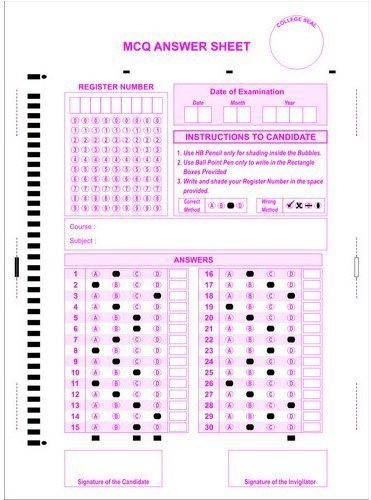
\includegraphics[width=14cm]{omrTemplate}\\
  \caption{Standard OMR template, \citet{stdTemplate}}%, 
  \label{fig:omrTemplate}
\end{figure}

In an OMR system there are normally two phases to marking an test, as stated in \citet{DraganI2003}. The first step is to determine the region within where the answers are located in the image. In this process the system finds the orientation of the template in the image and thus can approximate the location of the bubbles. Normally some preprocessing on a blank template is done beforehand too aid in locating the bubbles. Once the bubbles are found their locations gets stored and processed. The final step is then to calculate the average pixel concentration in the bubbles and estimate weather they have been filled in.

\section{Additional techniques}
\nomenclature[omrAcronym]{$OCR$}{Optical character recognition}
The above method allows for grading of tests using a simple OMR system. For the test grader used for the Applied Mathematics tests, there is needed to go beyond such a basic system.  In standard OCR, when a student makes a mistake, he/she needs to erase the existing answer and write a new answer in. This can be time consuming for a template with 8 bubble row choices per answer. This also increases the probability that the student will make a mistake in the process. Addressing this problem it is determined that two additional options needs to be made available. Firstly the student is allowed to cross out answers instead of totally erasing them. An example of this can be seen in Figure \ref{fig:Cross}. Then secondly the system needs to be accurate enough to determine the student's student number only by filling in the character blocks above the bubbles. This requirement will be addressed by using a PGM in Section \ref{sec:pgmStudentNum}. Using optical character recognition (OCR), the bubble information and character information can thus be cross-referenced in an intelligence way and will be implemented in Section \ref{sec:PGM}.

\begin{figure}
  \centering
  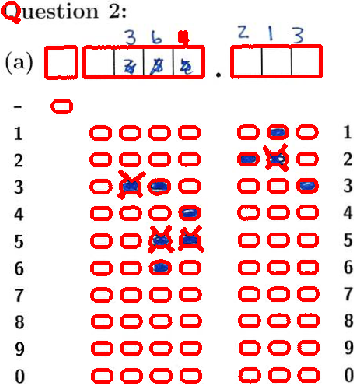
\includegraphics[width=5cm]{Cross}\\
  \caption{Example answer from student}
  \label{fig:Cross}
\end{figure}

\subsection{Contour detection}
To determine if an answer in a bubble is truly colored in and not just crossed out, contour detection is needed. This means that the contour around the bubble needs to be detected and used in analysis. In python this can be implemented using the freely available OpenCV library, as referenced in \citet{AdrianR2016}. OpenCV is an image processing library has has highly optimized techniques to find contours in a given image. With this information each bubble can be assessed not only by the pixels inside it, but also its shape. (Verander die image dalk na een wat 'n contour om het)

\subsection{Character recognition}
To further increase the accuracy of the system, Optical Character Recognition (OCR) software will also be need and applied on the characters blocks, present on the templates. Researched shows that one preferred way of doing OCR is using TensorFlow. This method is described in \citet{Tensor}. TensorFlow is also a python library, but allows the build of instructions to be implemented in ef{f}icient c++ code. For this test grader, TensorFlow will be used to setup a convolutional neural network. This network will read an image, containing the digit, and predict the probability of each digit.

\section{Conclusion: System requirements}

In conclusion it can be seen that the system will need to incorporate a combination of image processing on the bubbles and OCR on the digits handwritten by the students. Taking this combined evidence an more accurate result can be estimate, while also improving the convenience for students writing these test.
